\chapter{Threat Modeling}
Threat modeling is gaining more importance in application development, also known as the Secure Software Development Lifecycle (SSDLC) \citep{snyk_2022}. In the development cycle, one can use threat modeling approaches to identify and analyze different security issues in the application. Many other processes exist to carry out threat modeling, each of which has advantages and disadvantages. However, in this report, the Abuse Case Modelling and the STRIDE method will be used to analyze and recommend appropriate mitigations for the dangers using the recommended process from OWASP \citep{owasp_threat_model_process}.

\section{Threat Model Information}
\textbf{Application Name}: Appointment and Scheduling Management Information System
\textbf{Application Version}: 1.0 \newline
\textbf{Description}: Queens medical center is a community clinic that needs to replace its call-based appointment system with an online web application. Following the use cases (see. figure \ref{fig:usecase}), the application will have four actors/users.
\begin{itemize}
  \item Patients
  \item Receptionist
  \item Specialists/Doctors
  \item Admins
\end{itemize}

\newpage

\section{Trust Levels}
The trust levels define the privileges and grants an external entity/actors receive to use the application. The trust levels defined for the ASMIS system for the Queens medical center are defined in Table \ref{table:trust_levels}

\begingroup
\begin{table}[h!]
\centering
\setlength{\tabcolsep}{6.5pt} % Default value: 6pt
\renewcommand{\arraystretch}{1.8} % Default value: 1
\begin{tabular}{ |p{1cm}|p{6cm}|p{8cm}|}
 \hline
 \textbf{ID} & \textbf{Name} & \textbf{Description} \\ [0.5ex] 
 \hline
 1 & Anonymous Web User/Patient & A user who can schedule an appointment with a specialist without providing valid credentials. However, Personal Identifiable Information is provided during scheduling. \\
 \hline
 2 & Specialist with Valid Login Credentials & A special user who is a doctor/specialist in the clinic. When logged in using valid credentials, he/she can manage, create, modify, and view scheduling information connected to their profile. \\
 \hline
 3 & Receptionist with Valid Login Credentials & A special user who is a receptionist in the clinic. When logged in using valid credentials, he/she can manage, create, modify, and view the scheduling information of all patients. \\
 \hline
 4 & Admin with Valid Login Credentials & A special user who is an Admin in the clinic. When logged in using valid credentials, he/she can manage, create, modify, and view scheduling information connected to all specialist profiles. Additionally, the admin can add new specialists and assign permissions.\\
 \hline
 5 & Database Read/Write User & A database account is used to read and write the contents of the database.  \\ [1ex]
 \hline
\end{tabular}
\caption{Trust Levels ASMIS system.}
\label{table:trust_levels}
\end{table}
\endgroup

\section{Entry Points}
The entry points are the available access points through which users and potential hackers interact with the application. The definition of access points in the threat model aids us in determining from which points the attack vectors are carried out to hinder the application's functionality.\newline

\begingroup
\centering
\setlength{\tabcolsep}{6.5pt} % Default value: 6pt
\renewcommand{\arraystretch}{1.8} % Default value: 1
\begin{longtable}{ |p{3cm}|p{3cm}|p{5cm}| p{3cm} |}
 \hline
 \textbf{ID} & \textbf{Name} & \textbf{Description} & \textbf{Trust Levels} \\ [0.5ex] 
 \hline
 \multirow{2}{5em}{1} & Appointment Scheduling Main Page & The main page for all users of the application & (1) Anonymous Web User \\
 \hline
 \multirow{2}{5em}{2} & Appointment Scheduling Patient Page & The first point of contact for the patient to seek an appointment for their health issues. & (1) Anonymous Web User \\
 \hline
 3 & Login Page & The specialists, receptionists, and admins must log in before carrying out their respective functions & 
 (1)Specialist with Valid Login Credentials \newline
 (2)Receptionist with Valid Login Credentials \newline
 (3)Admin with Valid Login Credentials \newline
 (4)Database Read/Write User
 \\
 \hline
 4 & Appointment Management Page & The page can manage and modify all the information for appointments for a specific specialist & 
 (1)Specialist with Valid Login Credentials \newline
 (2)Receptionist with Valid Login Credentials \newline
 (3)Admin with Valid Login Credentials \newline
 (4)Database Read/Write User\\
 \hline
  5 & Search All Patient Pages & The page can manage and view all the information for patients who scheduled an appointment. & 
 (1)Specialist with Valid Login Credentials \newline
 (2)Receptionist with Valid Login Credentials \newline
 (3)Admin with Valid Login Credentials \newline
 (4)Database Read/Write User
 \\
 \hline
 6 & Admin Page & The page used by the admins to add new users and assign them with needed permissions & 
 (1)Admins with Valid Login Credentials \newline \\
 \hline
 \caption{Entry Points ASMIS system.}
    \label{table:entry_points}
\end{longtable}
\endgroup

\section{Abuse Case Model}

\begin{figure}[h!]
\centering
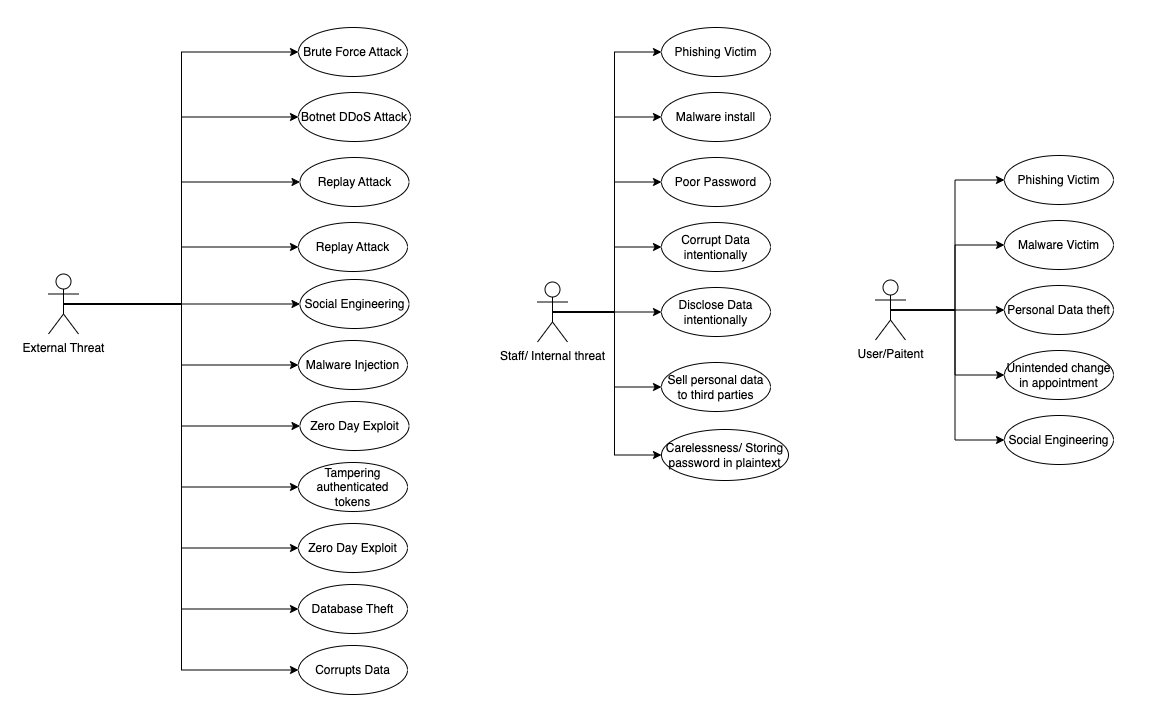
\includegraphics[width=\textwidth]{pics/abusecase.png}
\caption{Abuse case diagram for ASMIS}\label{fig:abuse_case}
\end{figure}

Using the Entry points (See Table \ref{table:entry_points}) and the use cases (See Figure\ref{fig:usecase}) the following possible abuse/misuse cases have been derived.
The possible dangers and the reliability of the ASMIS system are divided into three distinct actors: the external attacker, the staff/internal threat, and the patient/user. Table \ref{table:abuse_case} elaborates the risk factors with the recommended mitigation for the given abuse cases.

\begingroup
\centering
\setlength{\tabcolsep}{6.5pt} % Default value: 6pt
\renewcommand{\arraystretch}{1.8} % Default value: 1
\begin{longtable}{ |p{3cm}|p{3cm}|p{3cm}| p{5cm} |}
 \hline
 \textbf{Threat} & \textbf{Likelihood} & \textbf{Impact} & \textbf{Mitigations} \\ [0.5ex] 
 \hline
 Brute Force Attack & High & Moderate & (1) Block User for a while after X failed log in attempts\newline
 (2) Use fraud detection \newline
 (3) Use strong passwords
 \citep[p.~682-683]{herley2008protecting}\\
 \hline
 DDoS Attack & High & High & (1) Traffic flow Monitoring\newline
 (2) Anomaly Detection using ML \newline
 (3) Define strong and quick remedies in case of an attack
 \citep[p.~1]{DDOS}\\
\hline
   Malware & Moderate & High & (1) Install up-to-date antivirus.\newline
  (2) Use of threat monitoring tools, i.e., Security information and event management (SIEM) tools.\newline
  (3) Recurring Training - how to avoid malware  
  \\
 \hline
 Social Engineering & High & Moderate & (1) Security training and awareness for all users\newline
 (2) Incident Response \citep[p.~ 13-17]{chantler2008social}
  \\
  \hline
   Database Theft & Moderate & High & (1) Encrypt database at rest\newline
 (2) Database User credentials must be stored in a safe place
  \\
  \hline 
     Data corruption by staff & Low & High & (1) Work with least privileges\newline
 (2) Backup data in secure and isolated storage.
  \\
  \hline
       Poor password & High & High & (1) Strong password requirements\newline
       (2) Use MFA in complement with a password.
  \\
  \hline
 \caption{Abuse Case Risk and Mitigation Analysis}
    \label{table:abuse_case}
\end{longtable}
\endgroup

